% !TEX program = xelatex
% AY2016 材料力学 解答例（同志社 生命医科学 医工学コース 院試）
% 問題・図は 01_exams/2016/tex を土台に、参考/ の粒度で解答を付した。
\documentclass[11pt,a4paper]{article}
\usepackage{../../00_common/preamble}
\usetikzlibrary{positioning,arrows.meta,calc,patterns,decorations.pathmorphing}

\title{材料力学 AY2016 解答例（専門応用科目I）}
\author{}
\date{}

\begin{document}
\maketitle

\noindent\textbf{符号規約}：軸力 $N$・応力 $\sigma$ は引張りを正，部材の伸び（変位）$\lambda$ は伸長を正とする．
変位は上向きを正にとる．内圧を受ける薄肉円筒の応力は引張りを正とする．

%====================================================================
\section*{〔1〕}

図に示す組合せ棒について答える. 下面は固定され, 上面は剛体板で固定されている.
丸棒 1（下）と丸棒 2（上）は接点 X で接合され, 上面（剛体板）に外力 $P$（上向き）が作用する.
各部材の諸量は次のとおり（断面積，縦弾性係数，長さの順）.

\begin{center}
\begin{tikzpicture}[>=Latex,scale=0.95]
  % 地面（下面固定）
  \draw[thick] (-2.0,0) -- (2.0,0);
  \foreach \x in {-1.9,-1.6,...,1.95} {\draw (\x,0) -- (\x-0.25,-0.25);}
  % 剛体板（上面）
  \draw[line width=2pt] (-2.0,4.5) -- (2.0,4.5);
  % 円管3（外側2壁, 全長L）
  \fill[gray!20] (-1.6,0) rectangle (-1.3,4.5);
  \fill[gray!20] (1.3,0) rectangle (1.6,4.5);
  \draw (-1.6,0) rectangle (-1.3,4.5); \draw (1.3,0) rectangle (1.6,4.5);
  % 丸棒1（下, 3A, x:-0.7..0.7, y:0..2.25）
  \fill[gray!45] (-0.7,0) rectangle (0.7,2.25); \draw (-0.7,0) rectangle (0.7,2.25);
  % 丸棒2（上, A, x:-0.4..0.4, y:2.25..4.5）
  \draw (-0.4,2.25) rectangle (0.4,4.5);
  % 接点 X
  \fill (0,2.25) circle (1.6pt);
  \node[right] at (0.1,2.45) {X};
  % 番号
  \node at (0,1.1) {\large \textcircled{1}};
  \node at (0,3.4) {\large \textcircled{2}};
  \node at (1.45,2.4) {\large \textcircled{3}};
  % 外力 P（上向き）
  \draw[->,very thick] (0,4.5) -- (0,5.7) node[above]{$P$};
  % 剛体板ラベル
  \node[right] at (2.05,4.5) {\footnotesize 剛体板};
\end{tikzpicture}
\qquad
$\left(\begin{array}{llll}
  \text{丸棒}\,\text{\textcircled{1}} & 3A & 2E & L/2\\[2pt]
  \text{丸棒}\,\text{\textcircled{2}} & A & E & L/2\\[2pt]
  \text{円管}\,\text{\textcircled{3}} & 4A & 5E & L
\end{array}\right)$
\end{center}

\begin{enumerate}[label=(\arabic*)]
  \item 外力 $P$ を加えた場合に丸棒 1, 丸棒 2, 円管 3 に生じる内力 $N_1,N_2,N_3$,
        応力 $\sigma_1,\sigma_2,\sigma_3$, 変位 $\lambda_1,\lambda_2,\lambda_3$ を求めよ.
  \item $P=\SI{200}{kN}$, $E=\SI{100}{GPa}$, $L=\SI{1}{m}$, $A=\SI{100}{mm^2}$ のとき
        $\lambda_1,\lambda_2,\lambda_3$ を求めよ.
  \item 接点 X に外力 $F$ を負荷したとき丸棒 1 の応力が 0 となった. $F$ を求め,
        (2) の数値で $N_1\!\sim\!N_3$, $\sigma_1\!\sim\!\sigma_3$, $\lambda_1\!\sim\!\lambda_3$ を求めよ.
\end{enumerate}

\subsection*{解答}

\noindent\textbf{準備（剛性）}\quad 部材の軸剛性 $k=\dfrac{(\text{断面積})\times(\text{縦弾性係数})}{(\text{長さ})}$ は
\[
  k_1=\frac{3A\cdot 2E}{L/2}=\frac{12AE}{L},\qquad
  k_2=\frac{A\cdot E}{L/2}=\frac{2AE}{L},\qquad
  k_3=\frac{4A\cdot 5E}{L}=\frac{20AE}{L}.
\]

\medskip
\noindent\textbf{(1)}\quad 丸棒 1 と丸棒 2 は接点 X で直列につながり下面と剛体板を結ぶ（内側経路）．
円管 3 は同じく下面と剛体板を結ぶ（外側経路）．両経路は剛体板で結ばれるので，剛体板の上向き変位 $\delta$ を共有する（並列）．
直列の内側経路の剛性 $k_{\mathrm{in}}$ は
\[
  \frac{1}{k_{\mathrm{in}}}=\frac{1}{k_1}+\frac{1}{k_2}
  =\frac{L}{12AE}+\frac{6L}{12AE}=\frac{7L}{12AE}
  \;\Longrightarrow\; k_{\mathrm{in}}=\frac{12AE}{7L}.
\]
剛体板のつり合いは $P=(k_{\mathrm{in}}+k_3)\,\delta$．ここで
$k_{\mathrm{in}}+k_3=\dfrac{12AE}{7L}+\dfrac{140AE}{7L}=\dfrac{152AE}{7L}$ より
\[
  \ans{\;\delta=\frac{7PL}{152AE}\;}
\]
各経路の内力は，内側経路（直列なので $N_1=N_2$）が $N_{\mathrm{in}}=k_{\mathrm{in}}\delta$，円管 3 が $N_3=k_3\delta$．
\[
  N_1=N_2=\frac{12AE}{7L}\cdot\frac{7PL}{152AE}=\frac{3P}{38},\qquad
  N_3=\frac{20AE}{L}\cdot\frac{7PL}{152AE}=\frac{35P}{38}.
\]
\[
  \ans{\;N_1=N_2=\frac{3}{38}P,\qquad N_3=\frac{35}{38}P\;}
\]
応力は $\sigma=N/(\text{断面積})$ より
\[
  \ans{\;\sigma_1=\frac{N_1}{3A}=\frac{P}{38A},\qquad
        \sigma_2=\frac{N_2}{A}=\frac{3P}{38A},\qquad
        \sigma_3=\frac{N_3}{4A}=\frac{35P}{152A}\;}
\]
変位（伸び）は $\lambda=\dfrac{N\cdot(\text{長さ})}{(\text{断面積})\times(\text{縦弾性係数})}$ より
\[
  \lambda_1=\frac{N_1\cdot L/2}{3A\cdot 2E}=\frac{PL}{152AE},\quad
  \lambda_2=\frac{N_2\cdot L/2}{A\cdot E}=\frac{3PL}{76AE},\quad
  \lambda_3=\frac{N_3\cdot L}{4A\cdot 5E}=\frac{7PL}{152AE}.
\]
\[
  \ans{\;\lambda_1=\frac{PL}{152AE},\qquad \lambda_2=\frac{3PL}{76AE},\qquad \lambda_3=\frac{7PL}{152AE}\;}
\]
検算：内力の総和 $N_1+N_3=\dfrac{3P}{38}+\dfrac{35P}{38}=P$（$=$外力）✓．
また内側経路の伸び $\lambda_1+\lambda_2=\dfrac{PL}{152AE}+\dfrac{6PL}{152AE}=\dfrac{7PL}{152AE}$ は
円管 3 の伸び $\lambda_3$ および剛体板変位 $\delta$ に一致する（変位の適合）✓．

\medskip
\noindent\textbf{(2)}\quad $AE=\SI{100}{mm^2}\times\SI{100}{GPa}=\SI{1e7}{N}$ であり，
$\dfrac{PL}{AE}=\dfrac{200\times10^3\times 1}{1\times10^7}=\SI{0.02}{m}=\SI{20}{mm}$．これを (1) の各式へ代入して
\[
  \lambda_1=\frac{1}{152}\cdot 20=\SI{0.132}{mm},\quad
  \lambda_2=\frac{3}{76}\cdot 20=\SI{0.789}{mm},\quad
  \lambda_3=\frac{7}{152}\cdot 20=\SI{0.921}{mm}.
\]
\[
  \ans{\;\lambda_1\simeq\SI{0.132}{mm},\qquad \lambda_2\simeq\SI{0.789}{mm},\qquad \lambda_3\simeq\SI{0.921}{mm}\;}
\]
検算：$\lambda_1+\lambda_2=0.132+0.789=\SI{0.921}{mm}=\lambda_3$（剛体板変位に一致）✓．

\medskip
\noindent\textbf{(3)}\quad 接点 X の上向き変位を $u_X$，剛体板の上向き変位を $d_{\mathrm{top}}$ とおく．
各部材の内力は
\[
  N_1=k_1\,u_X,\qquad N_2=k_2\,(d_{\mathrm{top}}-u_X),\qquad N_3=k_3\,d_{\mathrm{top}}.
\]
丸棒 1 の応力が 0，すなわち $N_1=0$ なので $u_X=0$．
剛体板のつり合い $P=N_2+N_3=(k_2+k_3)\,d_{\mathrm{top}}$ より
\[
  d_{\mathrm{top}}=\frac{P}{k_2+k_3}=\frac{P}{\frac{2AE}{L}+\frac{20AE}{L}}=\frac{PL}{22AE},\quad
  N_2=k_2 d_{\mathrm{top}}=\frac{P}{11},\quad N_3=k_3 d_{\mathrm{top}}=\frac{10P}{11}.
\]
接点 X のつり合い（上向き正）は，丸棒 2 が X を上向きに $N_2$ で引き，丸棒 1 が X を下向きに $N_1$ で引き，外力 $F$ が加わるので
$N_2-N_1+F=0$．$N_1=0$ より $F=-N_2=-\dfrac{P}{11}$．
\[
  \ans{\;F=-\frac{P}{11}\quad(\text{すなわち大きさ }\tfrac{P}{11}\text{ の下向きの力})\;}
\]
このとき各量は（$N_1=0$ なので $\sigma_1=0,\ \lambda_1=0$）
\[
  N_1=0,\qquad N_2=\frac{P}{11},\qquad N_3=\frac{10P}{11},
\]
\[
  \sigma_1=0,\qquad \sigma_2=\frac{N_2}{A}=\frac{P}{11A},\qquad \sigma_3=\frac{N_3}{4A}=\frac{5P}{22A},
\]
\[
  \lambda_1=0,\qquad \lambda_2=\frac{N_2\cdot L/2}{A\cdot E}=\frac{PL}{22AE},\qquad
  \lambda_3=\frac{N_3\cdot L}{4A\cdot 5E}=\frac{PL}{22AE}.
\]
(2) の数値（$\dfrac{PL}{AE}=\SI{20}{mm}$, $A=\SI{100}{mm^2}$, $P=\SI{200}{kN}$）を代入すると
\[
  F=-\frac{200}{11}\simeq\SI{-18.2}{kN}\ (\text{下向き}),\quad
  N_2=\SI{18.2}{kN},\quad N_3=\SI{182}{kN},
\]
\[
  \sigma_2=\frac{P}{11A}\simeq\SI{182}{MPa},\quad \sigma_3=\frac{5P}{22A}\simeq\SI{455}{MPa},\quad
  \lambda_1=0,\quad \lambda_2=\lambda_3=\frac{20}{22}\simeq\SI{0.909}{mm}.
\]
\[
  \ans{\;F\simeq\SI{18.2}{kN}\ (\text{下向き}),\quad
        N_1=0,\ N_2=\SI{18.2}{kN},\ N_3=\SI{182}{kN},}
\]
\[
  \ans{\;\sigma_1=0,\ \sigma_2\simeq\SI{182}{MPa},\ \sigma_3\simeq\SI{455}{MPa},\quad
        \lambda_1=0,\ \lambda_2=\lambda_3\simeq\SI{0.909}{mm}\;}
\]
検算：$N_2+N_3=\dfrac{P}{11}+\dfrac{10P}{11}=P$（剛体板つり合い）✓．
また $\lambda_1+\lambda_2=0+\dfrac{PL}{22AE}=\dfrac{PL}{22AE}=\lambda_3=d_{\mathrm{top}}$（変位の適合）✓．

%====================================================================
\clearpage
\section*{〔2〕}

薄肉円筒（肉厚 $t$, 円筒外径 $d$: $t\ll d$）に内圧 $p$ が負荷されている.
円筒殻に生じる軸方向引張り応力 $\sigma_x$ と円周方向応力 $\sigma_\theta$ を求めよ.

\begin{center}
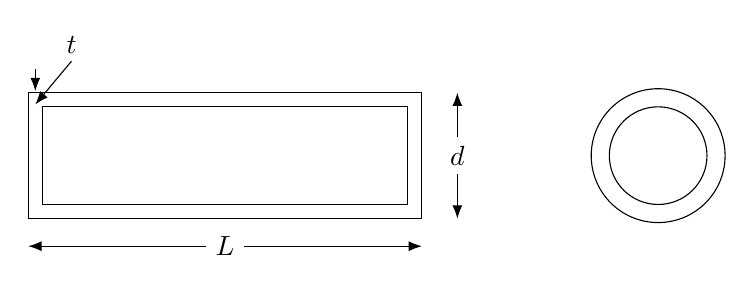
\begin{tikzpicture}[>=Latex]
  % 縦断面（薄肉円筒）
  \draw (0,0) rectangle (5,1.6);
  \draw (0.18,0.18) rectangle (4.82,1.42);
  % 肉厚 t
  \draw[->] (0.55,2.0) -- (0.09,1.45);
  \node at (0.55,2.2) {$t$};
  \draw[->] (0.09,1.9) -- (0.09,1.62);
  % 外径 d
  \draw[<->] (5.45,0) -- (5.45,1.6) node[midway,fill=white]{$d$};
  % 長さ L
  \draw[<->] (0,-0.35) -- (5,-0.35) node[midway,fill=white]{$L$};
  % 断面（円環）
  \begin{scope}[shift={(8.0,0.8)}]
    \draw (0,0) circle (0.85);
    \draw (0,0) circle (0.62);
  \end{scope}
\end{tikzpicture}
\end{center}

\subsection*{解答}

\noindent$t\ll d$ より直径 $d$ を平均直径とみなし，肉厚にわたる応力は一様とする（薄肉近似）．

\medskip
\noindent\textbf{軸方向応力 $\sigma_x$}\quad 円筒を軸に垂直な面で切断し，端のふたに作用する内圧と殻断面の引張り力のつり合いを考える．
内圧が端面に及ぼす軸方向の力は $p\cdot\dfrac{\pi d^2}{4}$，殻の断面積は（薄肉なので）$\pi d\,t$ である．つり合いより
\[
  \sigma_x\,(\pi d\,t)=p\cdot\frac{\pi d^2}{4}
  \;\Longrightarrow\;
  \ans{\;\sigma_x=\frac{p\,d}{4t}\;}
\]

\medskip
\noindent\textbf{円周方向応力 $\sigma_\theta$}\quad 軸を含む平面で円筒を縦に半分に切断し，軸方向長さ $L$ の半円殻のつり合いを考える．
内圧が投影面 $d\,L$ に及ぼす力は $p\,d\,L$，これを切断面 2 か所（各断面積 $t\,L$）の円周方向応力が支える．つり合いより
\[
  \sigma_\theta\,(2\,t\,L)=p\,(d\,L)
  \;\Longrightarrow\;
  \ans{\;\sigma_\theta=\frac{p\,d}{2t}\;}
\]

\medskip
検算：両者の比は $\sigma_\theta=2\,\sigma_x$ となり，薄肉円筒の周方向応力が軸方向応力の 2 倍という周知の結果に一致する ✓．

%====================================================================
\clearpage
\section*{〔3〕}

外径 $d$, 長さ $L$ の円形断面はり（固定端 A，自由端 B）の先端 B に長さ $L/2$ の剛体棒があり，
その先端に外力 $F$（はり軸に垂直な横荷重）が作用する．縦弾性係数・横弾性係数を $E,\ G$ とする．
点 $Q$ は固定端から測って $x=L-a$（自由端 B から距離 $a$），表面の最外縁
（$y=0,\ z=d/2$，曲げの引張り側）である．

\begin{center}
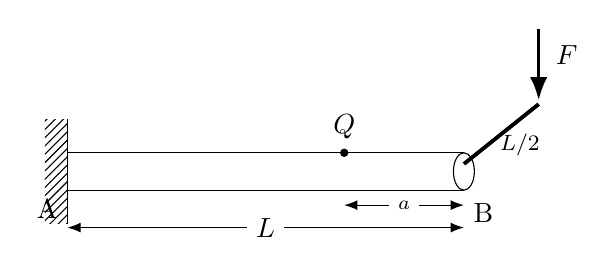
\begin{tikzpicture}[>=Latex,scale=0.95]
  % 固定壁
  \fill[pattern=north east lines] (0,-0.7) rectangle (0.3,0.7);
  \draw (0.3,-0.7) -- (0.3,0.7);
  % はり本体
  \draw (0.3,0.25) -- (5.6,0.25);
  \draw (0.3,-0.25) -- (5.6,-0.25);
  \draw (5.6,0) ellipse (0.14 and 0.25);
  \node[below left] at (0.3,-0.25) {A};
  \node[below right] at (5.6,-0.3) {B};
  % 点Q（上面, 引張り側）
  \fill (4.0,0.25) circle (1.6pt);
  \node[above] at (4.0,0.3) {$Q$};
  % 剛体腕とF
  \draw[line width=1.4pt] (5.6,0.1) -- (6.6,0.9);
  \node at (6.35,0.35) {\footnotesize $L/2$};
  \draw[->,very thick] (6.6,1.9) -- (6.6,0.95);
  \node[right] at (6.7,1.55) {$F$};
  % 寸法
  \draw[<->] (0.3,-0.75) -- (5.6,-0.75) node[midway,fill=white]{$L$};
  \draw[<->] (4.0,-0.45) -- (5.6,-0.45) node[midway,fill=white,font=\scriptsize]{$a$};
\end{tikzpicture}
\end{center}

剛体腕の横荷重 $F$ は，はり軸に対して
\emph{曲げモーメント}と\emph{ねじりトルク}の両方を点 $Q$ の断面に生じさせる
（曲げ＋ねじりの複合応力問題）．中実丸棒の断面定数は
\[
  I=\frac{\pi d^4}{64}\ (\text{断面二次モーメント}),\qquad
  I_p=\frac{\pi d^4}{32}\ (\text{断面二次極モーメント}).
\]

\subsection*{解答}

\noindent\textbf{(1)}\quad
点 $Q$ の断面（自由端 B から距離 $a$）に作用する曲げモーメントは，先端荷重 $F$ がモーメントの腕 $a$ をもつので
$M=F\,a$ である．最外縁 $z=d/2$ の曲げ応力（軸 $x$ 方向）は
\[
  \sigma_x=\frac{M\,(d/2)}{I}=\frac{F a\,(d/2)}{\pi d^4/64}
  \;\Longrightarrow\;
  \ans{\;\sigma_x=\frac{32\,F a}{\pi d^3}\quad(\text{引張り})\;}
\]
中実丸棒には円周方向の垂直応力は生じないので
\[
  \ans{\;\sigma_y=0\;}
\]

\medskip
\noindent\textbf{(2)}\quad
剛体腕のオフセット $L/2$ によって，はり軸まわりにねじりトルク
$T=F\cdot\dfrac{L}{2}$ が生じる．表面のせん断応力は
\[
  \tau_{xy}=\frac{T\,(d/2)}{I_p}=\frac{(FL/2)\,(d/2)}{\pi d^4/32}
  \;\Longrightarrow\;
  \ans{\;\tau_{xy}=\frac{8\,F L}{\pi d^3}\;}
\]
なお点 $Q$ は断面の最外縁にあり，横せん断力 $F$ によるせん断応力はそこで $0$ になるため，
$Q$ 点のせん断応力はねじり分のみが残る．

\medskip
\noindent\textbf{(3)}\quad
点 $Q$ は $\sigma_x$（引張り），$\sigma_y=0$，$\tau_{xy}$ の平面応力状態にある．モール応力円は
中心 $\left(\dfrac{\sigma_x}{2},\,0\right)$，半径 $R=\sqrt{\left(\dfrac{\sigma_x}{2}\right)^2+\tau_{xy}^{\,2}}$ の円となる．ここで
\[
  \frac{\sigma_x}{2}=\frac{16\,F a}{\pi d^3},\qquad
  R=\sqrt{\left(\frac{16Fa}{\pi d^3}\right)^2+\left(\frac{8FL}{\pi d^3}\right)^2}
   =\frac{8F}{\pi d^3}\sqrt{4a^2+L^2}.
\]

\begin{center}
\begin{tikzpicture}[>=Latex,scale=1.0]
  \def\cx{2.6}   % 中心 σx/2
  \def\R{1.9}    % 半径
  % 軸
  \draw[->] (-0.4,0) -- (6.0,0) node[right]{$\sigma$};
  \draw[->] (0,-2.4) -- (0,2.4) node[above]{$\tau$};
  % モール円
  \draw[thick] (\cx,0) circle (\R);
  \fill (\cx,0) circle (1.2pt);
  \node[below right] at (\cx,-0.05) {\footnotesize $\dfrac{\sigma_x}{2}$};
  % 点 Q (σx, τxy) と (σy=0, -τxy)
  \fill (4.5,1.1) circle (1.4pt); \node[above right] at (4.5,1.1) {\footnotesize $(\sigma_x,\tau_{xy})$};
  \fill (0.7,-1.1) circle (1.4pt); \node[below left] at (0.7,-1.1) {\footnotesize $(0,-\tau_{xy})$};
  \draw (4.5,1.1) -- (0.7,-1.1);
  % 主応力
  \fill (\cx-\R,0) circle (1.2pt); \node[above left] at (\cx-\R,0) {\footnotesize $\sigma_2$};
  \fill (\cx+\R,0) circle (1.2pt); \node[above right] at (\cx+\R,0) {\footnotesize $\sigma_1$};
  % τmax
  \draw[<->] (\cx,0.06) -- (\cx,\R-0.02);
  \node[right] at (\cx+0.05,\R/2) {\footnotesize $\tau_{\max}=R$};
\end{tikzpicture}
\end{center}

\noindent 主応力 $\sigma_1,\sigma_2$ と最大せん断応力 $\tau_{\max}$ は
\[
  \sigma_{1}=\frac{\sigma_x}{2}+R,\qquad
  \sigma_{2}=\frac{\sigma_x}{2}-R,\qquad
  \tau_{\max}=R=\frac{8F}{\pi d^3}\sqrt{4a^2+L^2}.
\]
最大主応力は $\sigma_{\max}=\sigma_1$ であり，
\[
  \sigma_{\max}=\frac{16Fa}{\pi d^3}+\frac{8F}{\pi d^3}\sqrt{4a^2+L^2}
  \;\Longrightarrow\;
  \ans{\;\sigma_{\max}=\frac{8F}{\pi d^3}\Bigl(2a+\sqrt{4a^2+L^2}\Bigr)\;}
\]
検算：$\sigma_1+\sigma_2=\sigma_x$（応力の不変量），かつ
$\sigma_1\sigma_2=\left(\dfrac{\sigma_x}{2}\right)^2-R^2=-\tau_{xy}^{\,2}$
（$\sigma_y=0$ のときの関係）を満たす ✓．

\medskip
\noindent\textbf{(4)}\quad
円形断面はりを〔2〕のような薄肉円筒に置きかえても，曲げ・ねじりの応力公式の形は変わらない．
断面二次モーメントを $I_z$，断面二次極モーメントを $I_p$ として，曲げモーメント $M=Fa$，
ねじりトルク $T=FL/2$，最外縁 $d/2$ を用いると
\[
  \sigma_x=\frac{M\,(d/2)}{I_z}=\frac{F a\,d}{2\,I_z},\qquad
  \sigma_y=0,\qquad
  \tau_{xy}=\frac{T\,(d/2)}{I_p}=\frac{F L\,d}{4\,I_p}.
\]
\[
  \ans{\;\sigma_x=\frac{F a\,d}{2 I_z},\qquad \sigma_y=0,\qquad \tau_{xy}=\frac{F L\,d}{4 I_p}\;}
\]
検算：中実丸棒の値 $I_z=I=\dfrac{\pi d^4}{64}$，$I_p=\dfrac{\pi d^4}{32}$ を代入すると
$\sigma_x=\dfrac{32Fa}{\pi d^3}$，$\tau_{xy}=\dfrac{8FL}{\pi d^3}$ となり，(1)(2) に一致する ✓．

\end{document}
